\documentclass[a4paper]{article}


\usepackage{amsmath} % using math package
\usepackage{amssymb}
\usepackage{xcolor}
\usepackage{graphicx}

%define new command
\newcommand{\pd}{\partial}


\newcommand{\ket}[1]{\big|  #1 \big \rangle }
\newcommand{\bra}[1]{ \big\langle #1 \big | }

\newcommand {\avg}[3] {\langle {#1} |{ #2} |{#3} \rangle} 


\begin{document}
\title{Explain Stern-Gerlach Experiment With Quantum Measurement}
\author{Youyang Zhou\\Yunnan University}
\date{17 Sep, 2018}
\maketitle

\begin{abstract}
Stern-Gerlach experiment is an important experiment in quantum mechanics. We understand the phenomenon of Stern-Gerlach experiment by analogy with the polarization experiment of light, and using quantum measurement, 
\textcolor{red}{explain the Stern-Gerlach experiment}.  
\end{abstract}

\section{Introduction}
Since the publication of De Broglie's doctoral thesis in 1924, quantum mechanics has been established. Quantum mechanics is the basic theory of the microscopic world. Bohr once said, "Those who are not shocked by the theory of quantum mechanics do not understand quantum mechanics".
Up to now, quantum mechanics has played a huge role in scientific research, such as condensed matter physics, quantum information, biophysics, chemical physics, laser physics and so on. Professoer Anthony J. Leggett gave his answer to “What do people think about quantum mechanics a thousand years later” that “One possibility: he assured me that even in the year 3000, people still believed that quantum mechanics was basically a complete description of the physical world. Another possibility: travelers returning from the third millennium tell me that no one believes in quantum mechanics anymore.I personally prefer this view.”
One of the most important experiments in quantum mechanics is the Stern-Gerlach experiment. How to comprehend this phenomenon is very helpful for us to learn quantum mechanics.
We want to understand the phenomenon of Stern-Gerlach experiment by analogy with the polarization experiment of light, and use quantum measurement to explain the Stern-Gerlach experiment mathematically in the form of the Dirac symbol.
 
\section{Methods}
As we know, what we observe experimentally in Stern-Gerlach experiment is more like the situation in Figure 1. 
\begin{figure}[htbp!] \label{experiment}
\centering % put the fig. in the center
    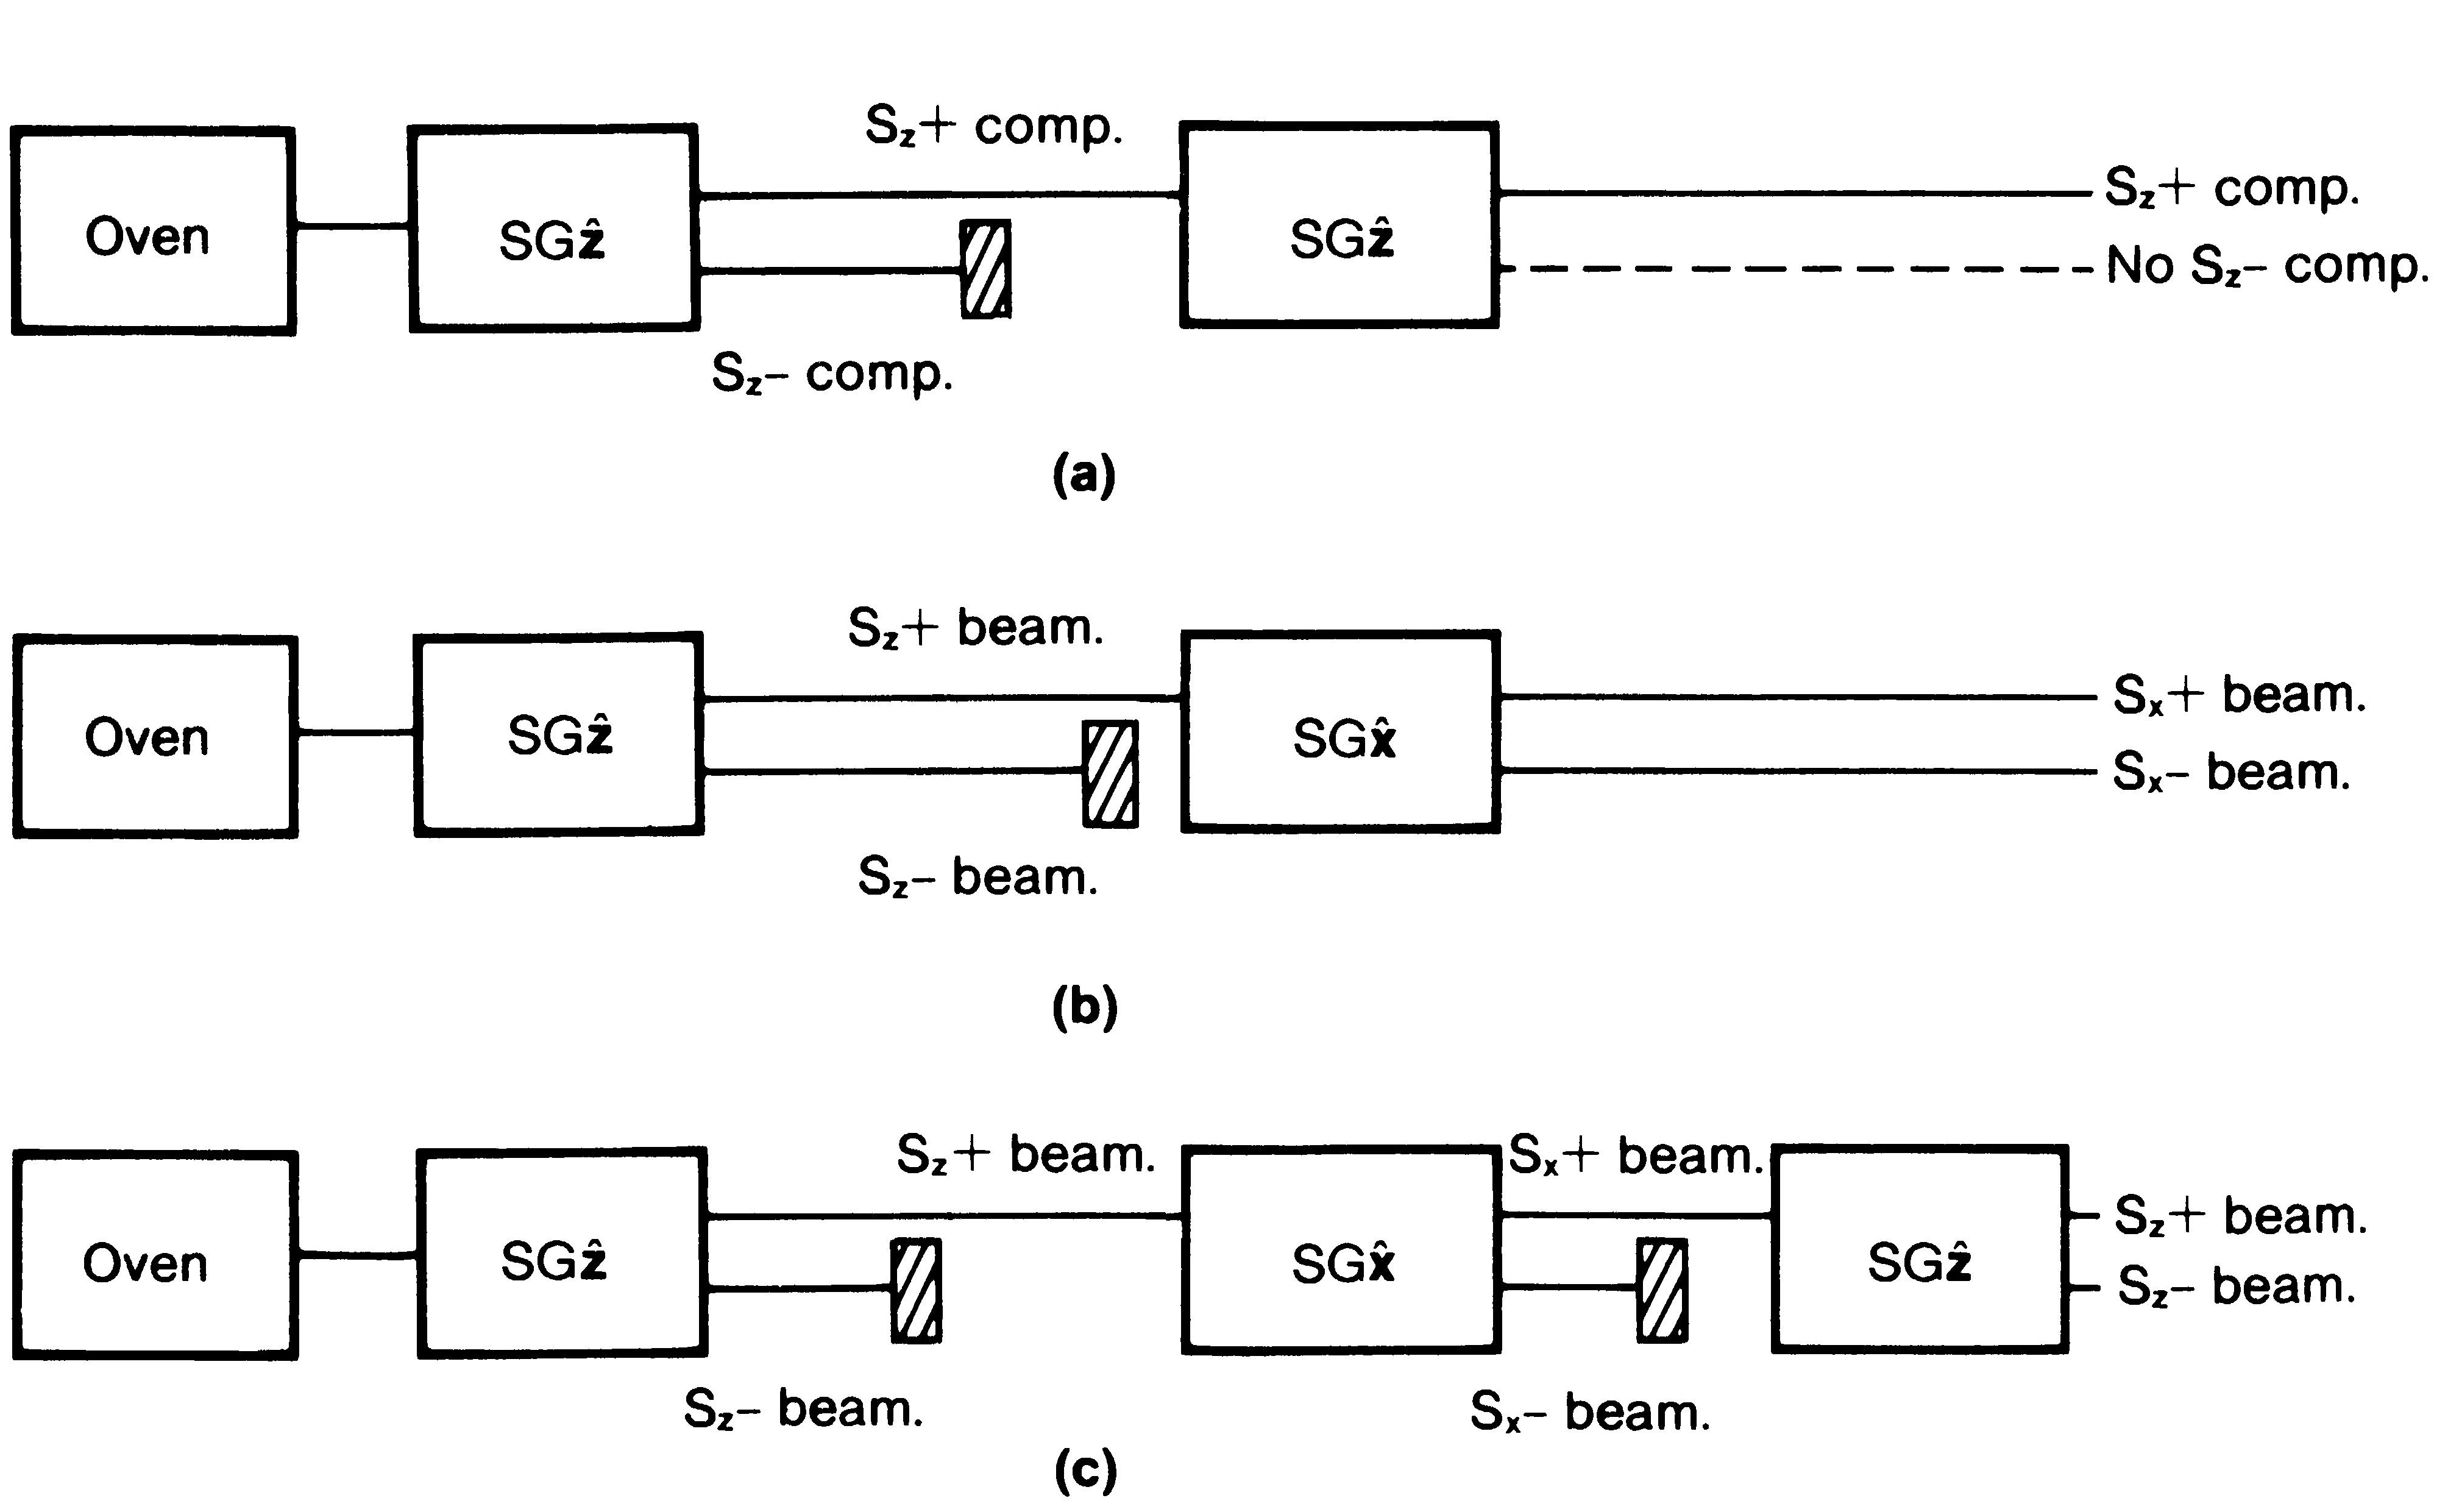
\includegraphics[width=0.5\linewidth]{SGexperiment.jpg}
    \caption{Sequential Stern-Gerlach experiment}
\end{figure}
\cite{Stern1922}The first arrangement we consider is relatively straightforward. We subject the beam coming out of the oven to the arrangement, where SG$\hat{z}$ stands for an apparatus with the inhomogeneous magnetic field in the $z$-direction. We then block the S$_z$- component coming out of the first SG$\hat{z}$ apparatus and let the remaining S$_z$+ component be subjected to another SG$\hat{z}$ apparatus. This time there is only one beam component coming out of the second apparatus--just the S$_z$+ component. This is perhaps not so surprising; after all if the atom spins are up, they are remain so. The second arrangement is interesting shown in Figure 1.b. The S$_z$+ beam that enters the second apparatus (SG$\hat{x}$) is now split into two components, an S$_x$+ component and an S$_x$- component, with equal intensities. The third step is shown in Figure 1(c), which most dramatically illustrates the peculiarities of quantum-mechanical systems. This time we add to the arrangement of Figure 1(b) yet a third apparatus,  of the SG$\hat{z}$ type. It is observed experimentally that two components emerge from the third apparatus, not one; the emerging beams are seen to have both an S$_z$+ component and an S$_z$- component. It is hard to understand this in classical mechanics. However in polarization of light, we can seek the similar  situation shown in Figure 2. 
\begin{figure}[htbp!] \label{polarization}
\centering % put the fig. in the center
    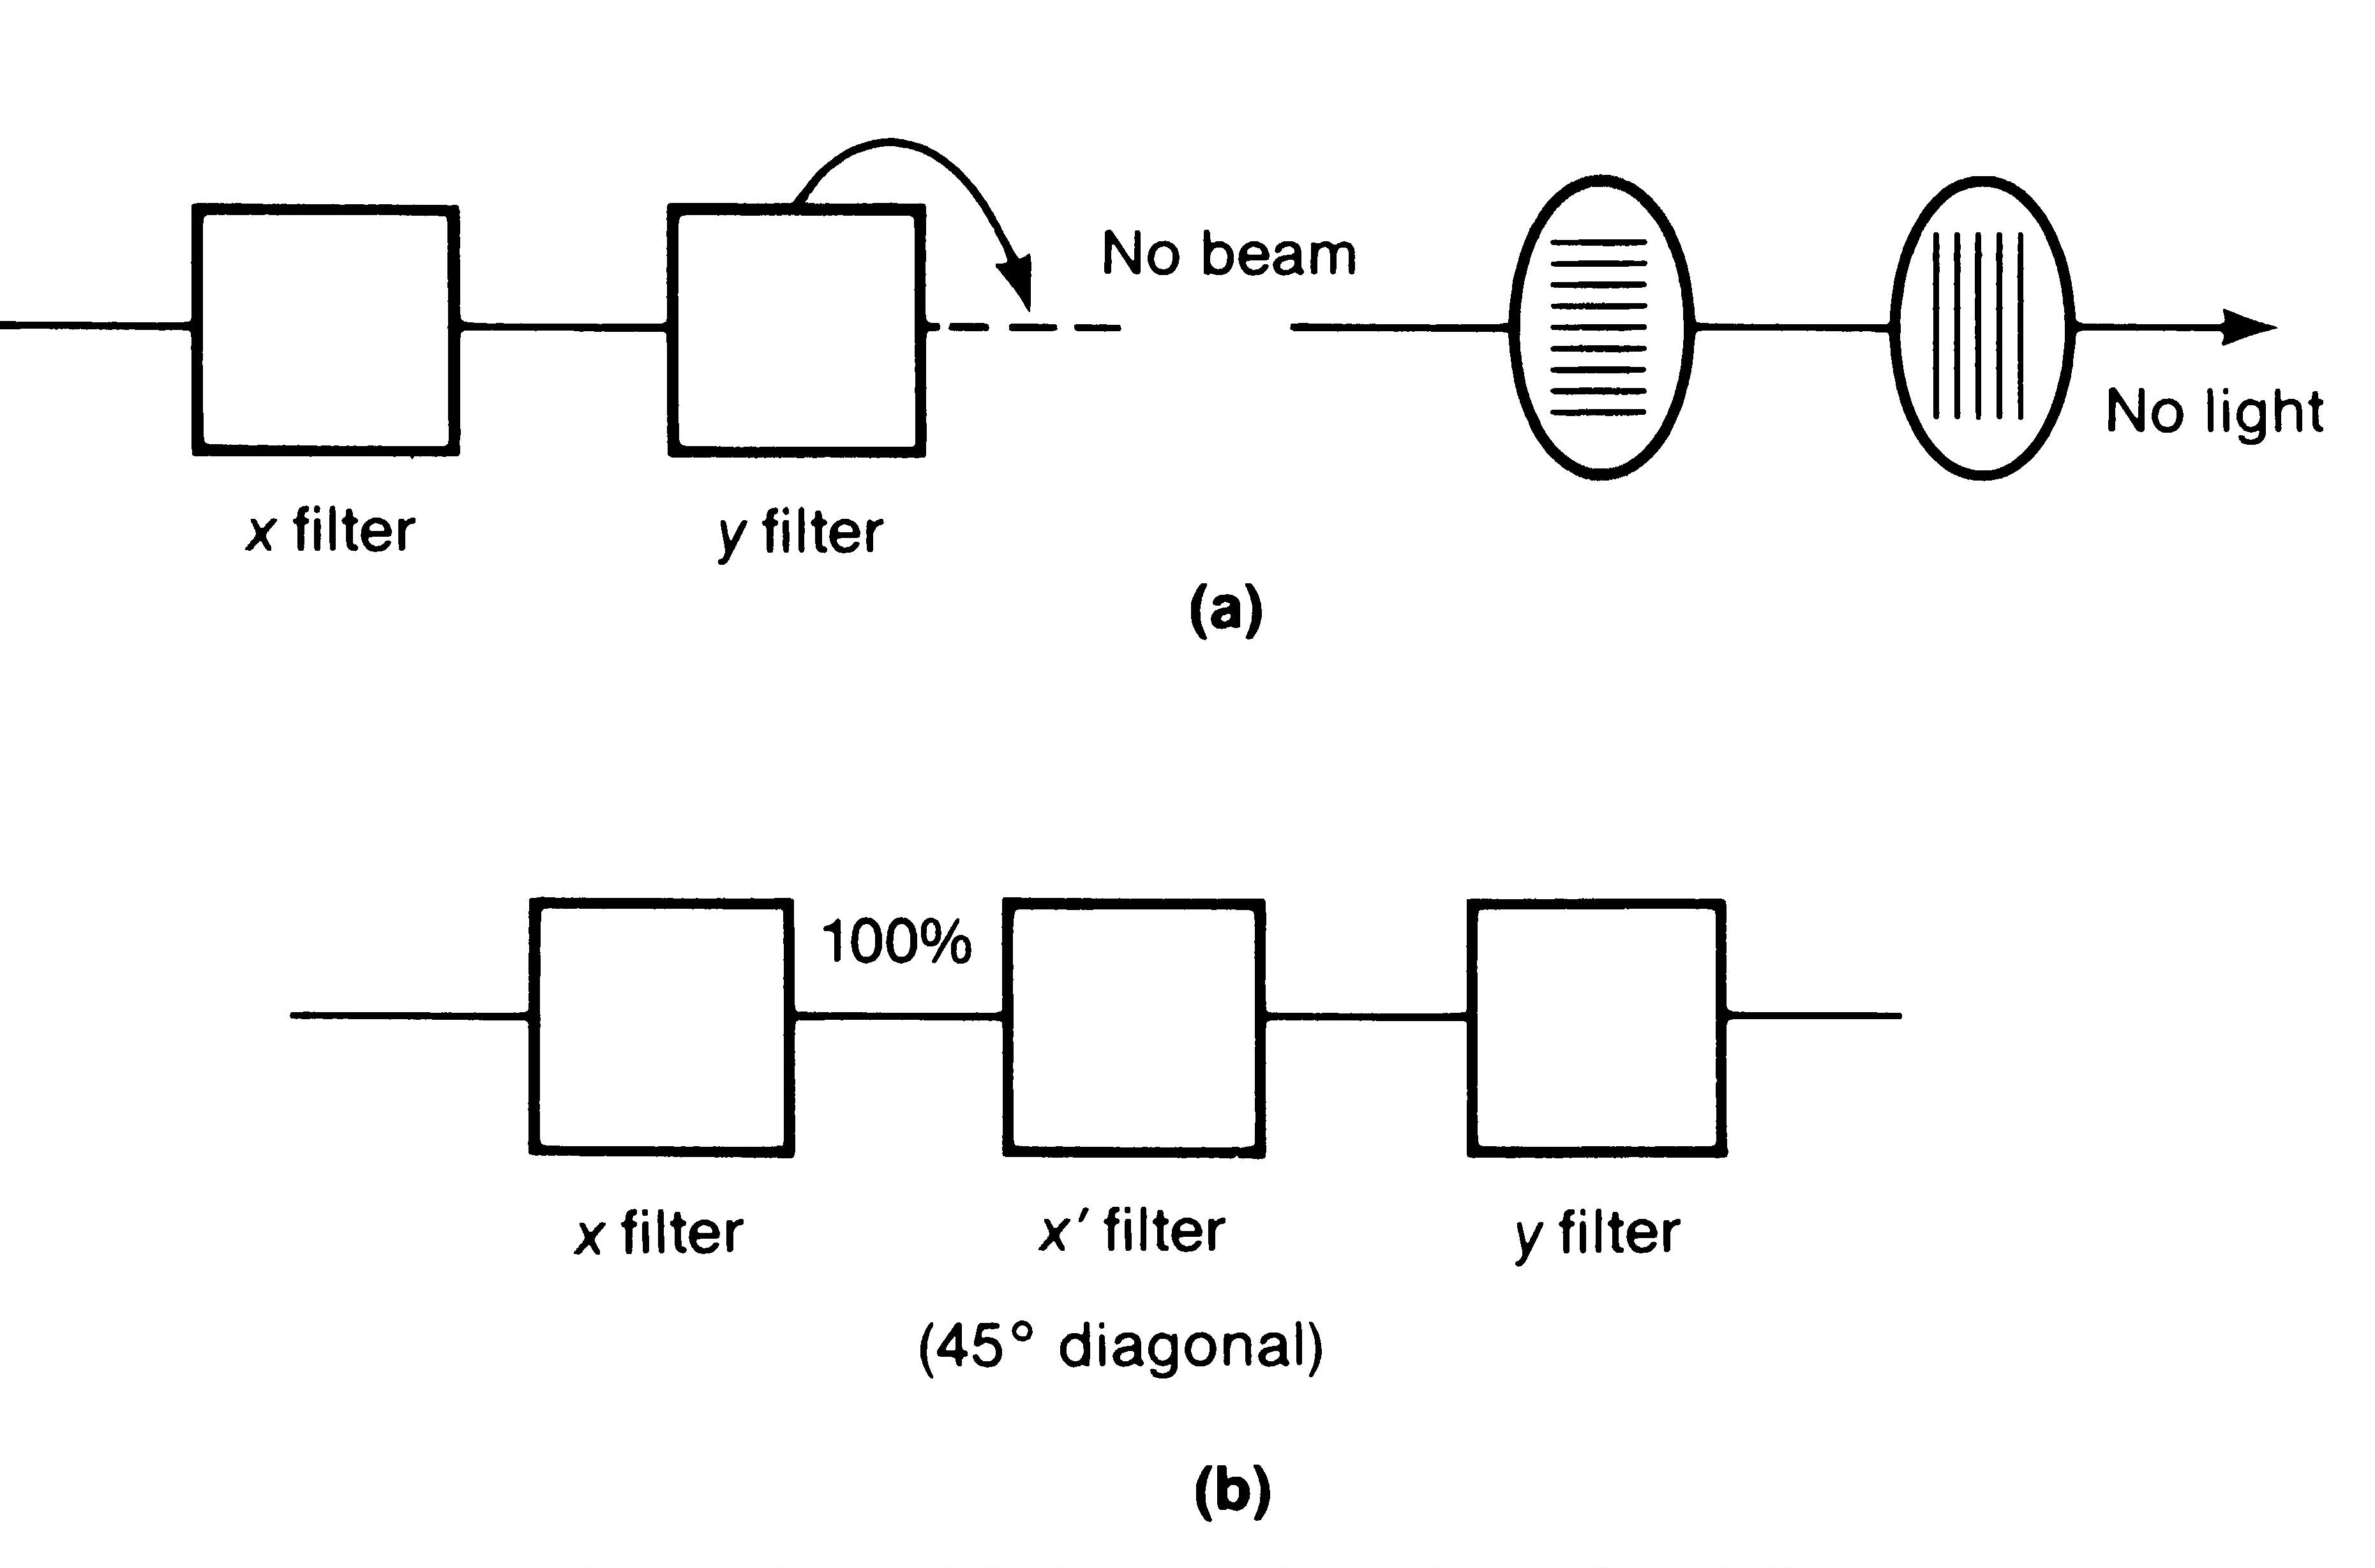
\includegraphics[width=0.5\linewidth]{polarization.jpg}
    \caption{Light beams subjected to Polaroid filters}
\end{figure}
It is well known that when we let a light beam go through an $x$-filter and subsequently let it impinge on a $y$-filter, no light beam comes out provided. What is similar, we insert between the $x$-filter and the $y$-filter yet another Polaroid that selects only a beam polarized in the direction--which we call the $x'$-direction--that makes an angle of 45° with the $x$-direction in the xy plane. This time,  there is a light beam coming out of the $y$-filter despite the fact that right after the beam went through the $x$-filter it did not have any polarization component in the $y$-direction. In other words, once the $x'$-filter intervenes and selects the $x'$-polarized beam, it is immaterial whether the beam was previously $x$-polarized. The selection of the $x'$-polarized beam by the second Polaroid destroys any previous information on light polarization, which is quite analogous to the situation that we encountered earlier with the SG arrangement of Figure 1(b).
In optics, we have explain this experiment. As shown in Figure 3.
\begin{figure}[htbp!] \label{x'and y'}
\centering % put the fig. in the center
    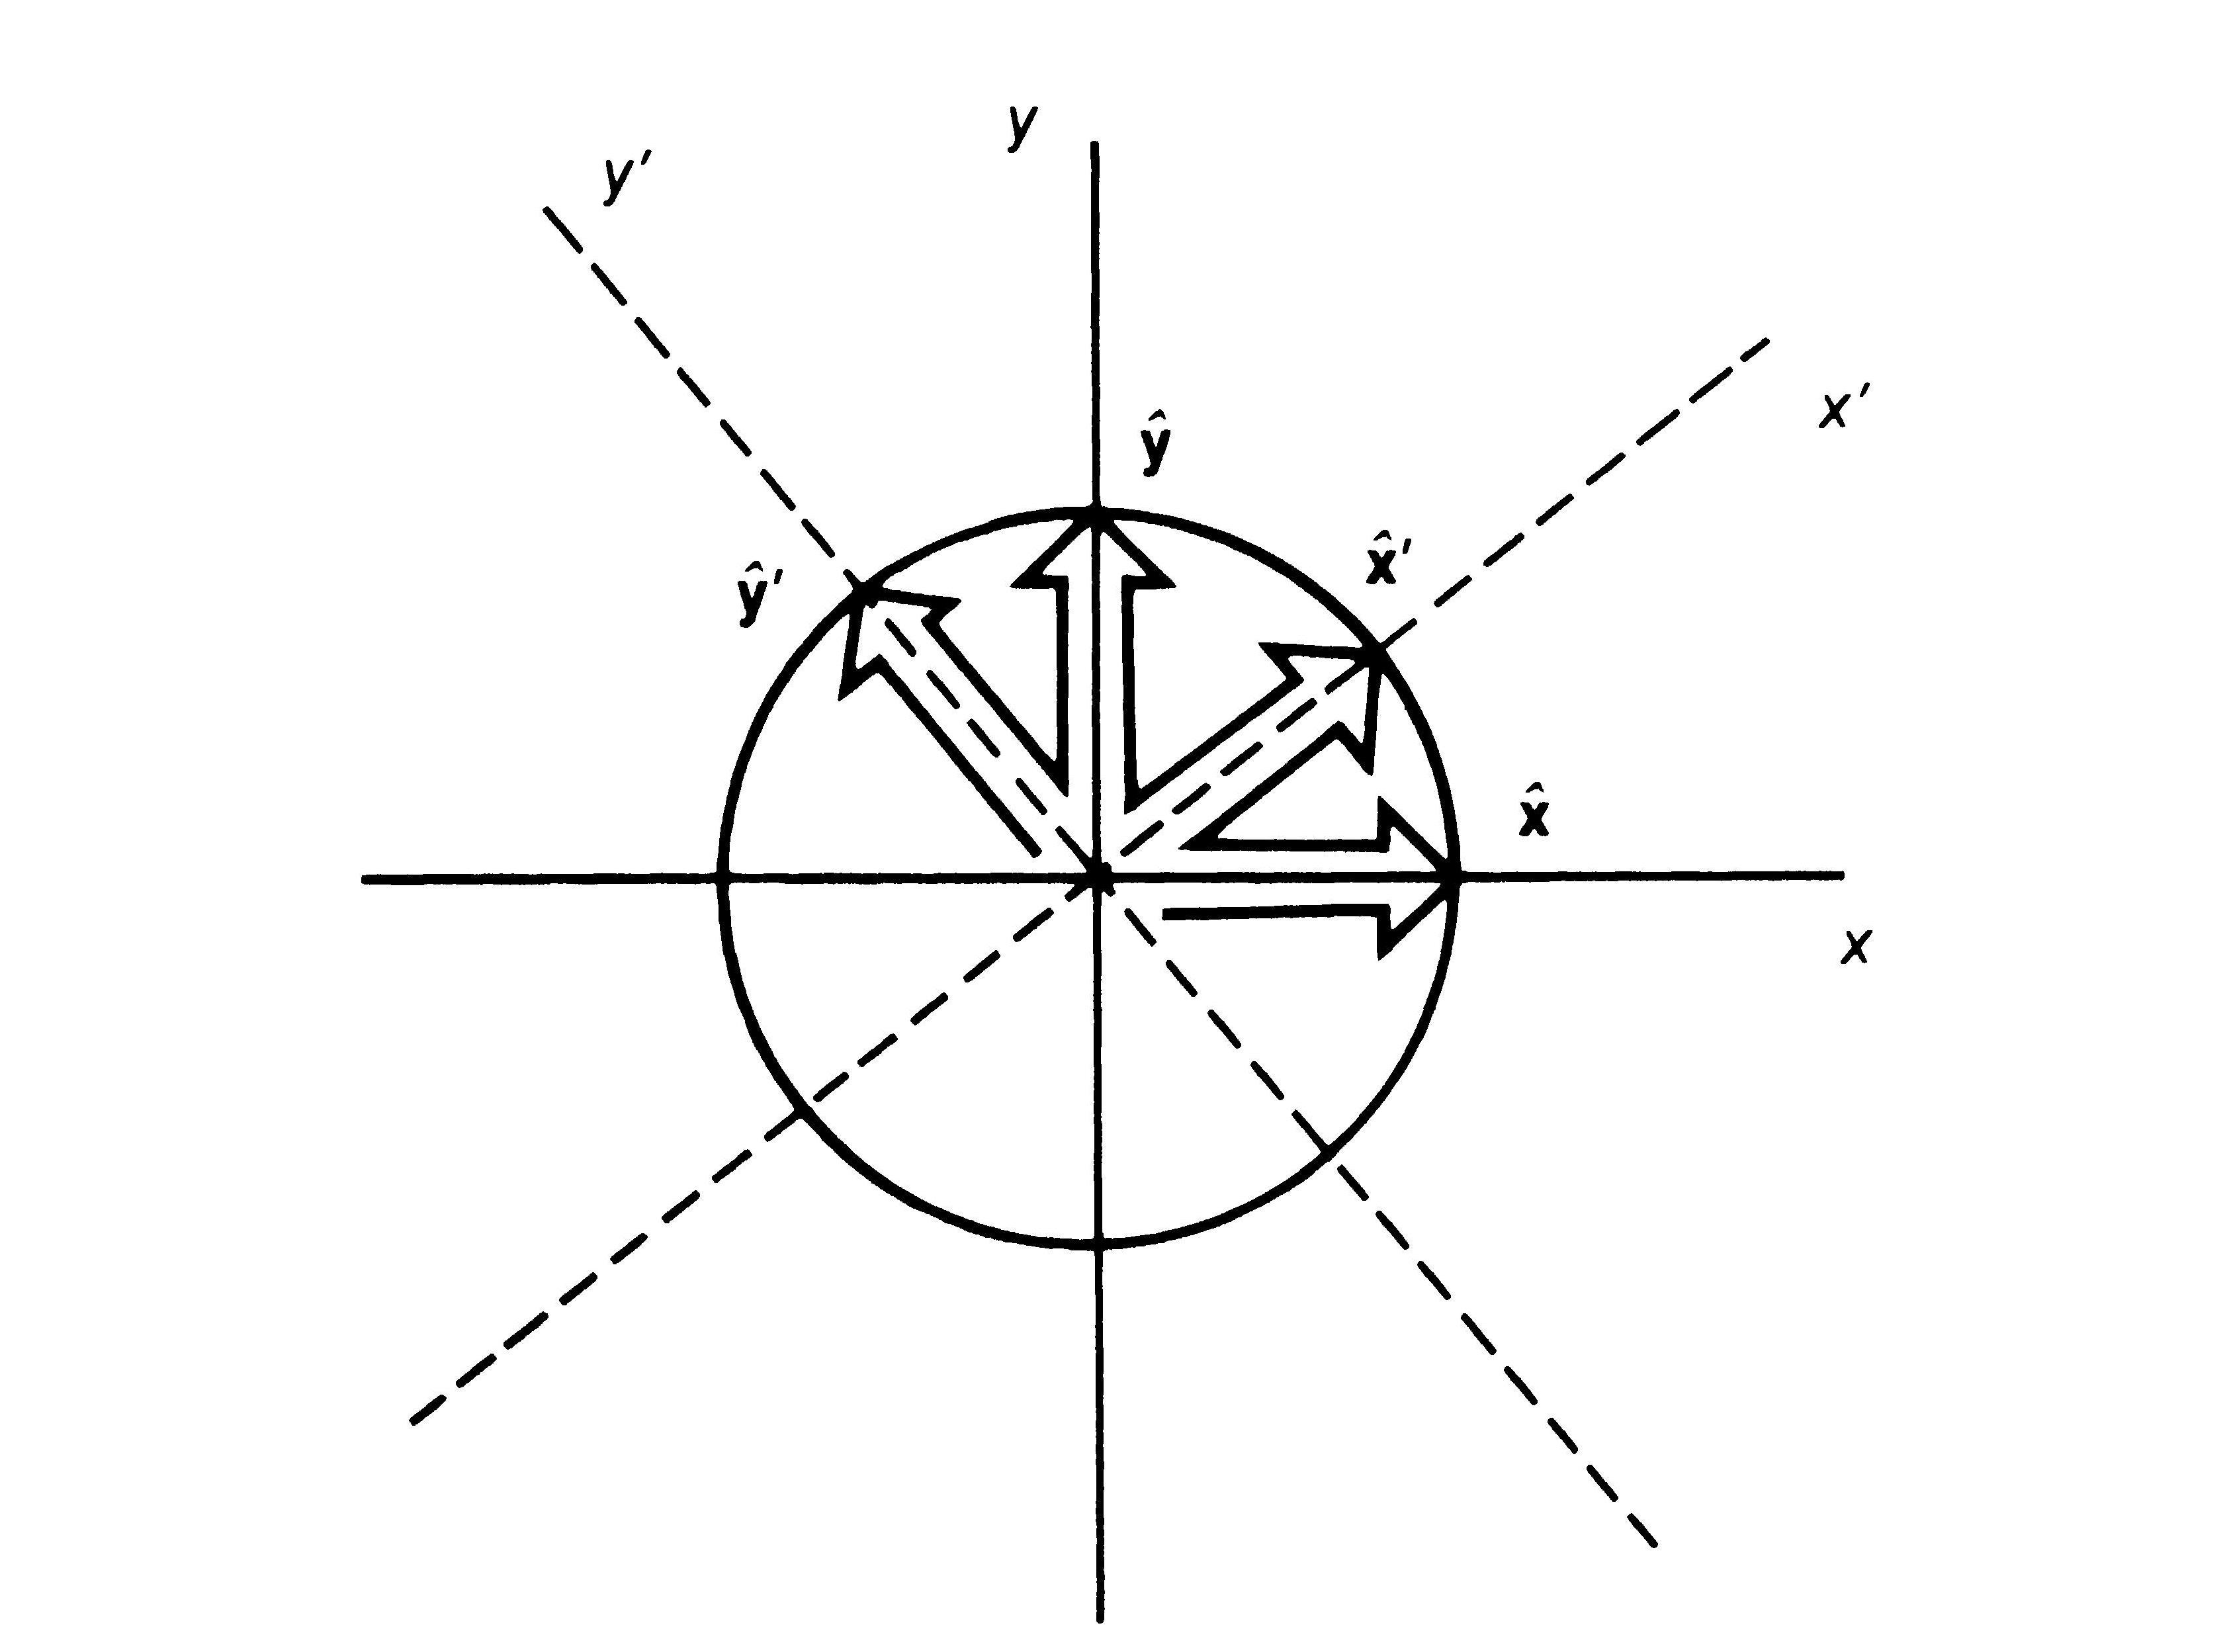
\includegraphics[width=0.5\linewidth]{change axes.jpg}
    \caption{Orientations of the $x'$- and $y'$-axes}
\end{figure}
We can get that
\begin{eqnarray}
E_0 \hat{x} ' \cos(kz-\omega t) = E_0 [ \dfrac{1}{\sqrt{2}} \hat{x} \cos(kz-\omega t) + \dfrac{1}{\sqrt{2}} \hat{y} \cos(kz-\omega t) ],\\
E_0 \hat{y} ' \cos(kz-\omega t) = E_0 [ - \dfrac{1}{\sqrt{2}} \hat{x} \cos(kz-\omega t) + \dfrac{1}{\sqrt{2}} \hat{y} \cos(kz-\omega t) ].
\end{eqnarray}
So we can comprehen the experiment of Figure 2(b). And just as $\hat{x}$ and $\hat{y}$ are the base vectors used to decompose the polarization vector $\hat{x}'$ of the $\hat{x}'$-polarized light, it is reasonable to represent the S$_x$+ state by a vector. We denote this vector by $\vert S_x;+\rangle$ and write it as a linear combination of two base vectors, $\vert S_z;+\rangle$ and $\vert S_z;+\rangle$, which correspond to the S$_z$+ and the S$_z$- states. So we guess the equation.
\begin{eqnarray}
\ket{S_x;+} = \dfrac{1}{\sqrt{2}} \ket{S_z;+} + \dfrac{1}{\sqrt{2}} \ket{S_z;-}\\
\ket{S_x;-} = -\dfrac{1}{\sqrt{2}} \ket{S_z;+} + \dfrac{1}{\sqrt{2}} \ket{S_z;-}\\
\end{eqnarray}


\section{Results}
What we would do next is calculate the equation with measurement. 
At first, what we obtain in the experiment is probability for every state we measured. So the first thing we need to figure out is the expression of probability. For a start state $\phi$ and finish state $\chi$, the probability is 
\begin{equation}
P = {| \langle \chi | \phi \rangle |}^2
\end{equation}
And we have known that the probability for the S$_x$+ state to be thrown into $\ket{S_z;\pm}$, simply denoted as $\ket{\pm}$, is $ \dfrac{1}{2} $ each. 
\begin{equation}
{| \langle + | S_x;+ \rangle |}^2 = {| \langle - | S_x;+ \rangle |}^2 = \dfrac{1}{2}
\end{equation}
We can therefore construct the S$_x$+ ket as follows:
\begin{equation}
\ket{S_x;+} = \dfrac{1}{\sqrt{2}} \ket{+} + \dfrac{1}{\sqrt{2}} e^{i\delta_1} \ket{-}
\end{equation}
with $\delta_1$ real. Because the S$_X$- ket must be orthogonal to the S$_x$+ ket , we can  construct the S$_x$- ket:
\begin{equation}
\ket{S_x;+} = \dfrac{1}{\sqrt{2}} \ket{+} - \dfrac{1}{\sqrt{2}} e^{i\delta_1} \ket{-}
\end{equation}
So the operator $\hat{S}_x$ is
\begin{equation}
\begin{aligned}
\hat{S}_x &= \dfrac{\bar{h}}{2} [ (\ket{S_x;+} \bra{S_x;+}) - (\ket{S_x;-} \bra{S_x;-}) ]\\
&= \dfrac{\bar{h}}{2} [ e^{-i \delta_1} (\ket{+} \bra{+}) - e^{i \delta_1} (\ket{-} \bra{-}) ]
\end{aligned}
\end{equation}
In a similar way,
\begin{equation}
\begin{aligned}
\ket{S_y;\pm} &= \dfrac{1}{\sqrt{2}} \ket{+} \pm \dfrac{1}{\sqrt{2}} e^{i\delta_2} \ket{-}\\
\hat{S}_y &= \dfrac{\bar{h}}{2} [ e^{-i \delta_2} (\ket{+} \bra{+}) - e^{i \delta_2} (\ket{-} \bra{-}) ]
\end{aligned}
\end{equation}
How can we determine $\delta_1$ and $\delta_2$? Suppose we have a beam of spin $\dfrac{1}{2}$ atoms moving in the $z$-direction. We can consider a sequential Stern-Gerlach experiment with SG$\hat{x}$ followed by SG$\hat{y}$. According to the result
\begin{equation}
{| \langle S_y; \pm | S_x;+ \rangle |} = {| \langle S_y; \pm | S_x;- \rangle |} = \dfrac{1}{\sqrt{2}}
\end{equation}
input (9)(11) into (12), we obtain
\begin{equation}
\dfrac{1}{2} [ 1 \pm e^{i( \delta_1 - \delta_2)} ] = \dfrac{1}{\sqrt{2}}
\end{equation}
which is satistied only if 
\begin{equation}
\delta_1 - \delta_2 = \pi / 2 \	or	- \pi / 2
\end{equation}
Because it is convenient to take the S$_x$ matrix elements to be real, so we can set $\delta_1$ = 0, and $\delta_2$ = $\pi$/2. Finally we have
\begin{eqnarray}
\ket{S_x;\pm} = \dfrac{1}{\sqrt{2}} \ket{+} \pm \dfrac{1}{\sqrt{2}} \ket{-}\\
\ket{S_y;\pm} = \dfrac{1}{\sqrt{2}} \ket{+} \pm \dfrac{i}{\sqrt{2}} \ket{-}
\end{eqnarray}
and
\begin{eqnarray}
\begin{aligned}
\hat{S}_x &= \dfrac{\bar{h}}{2} (\ket{+} \bra{+}) + (\ket{-} \bra{-}) ]\\
\hat{S}_y &= \dfrac{\bar{h}}{2} (\ket{+} \bra{+}) + i (\ket{-} \bra{-}) ]
\end{aligned}
\end{eqnarray}

\section{Conclusion}
Stern-Gerlach experiment only have dealed with a simple system, which contains spin $\dfrac{1}{2}$ particle and calculated the spin operator expression. However we can learn the methods of quantum measurement to work with some complex systems. And in a similar system, we can do some calculation and prediction, if we have some operator expression obtained by quantum measurement based on the experimental results.
\bibliographystyle{plain}
\bibliography{SG.Bib}

\end{document}
